
\chapter{Roadmap} 
\label{ch:Chapter5}
\vfill \minitoc \newpage

\begin{figure}[!ht]
	\centering
	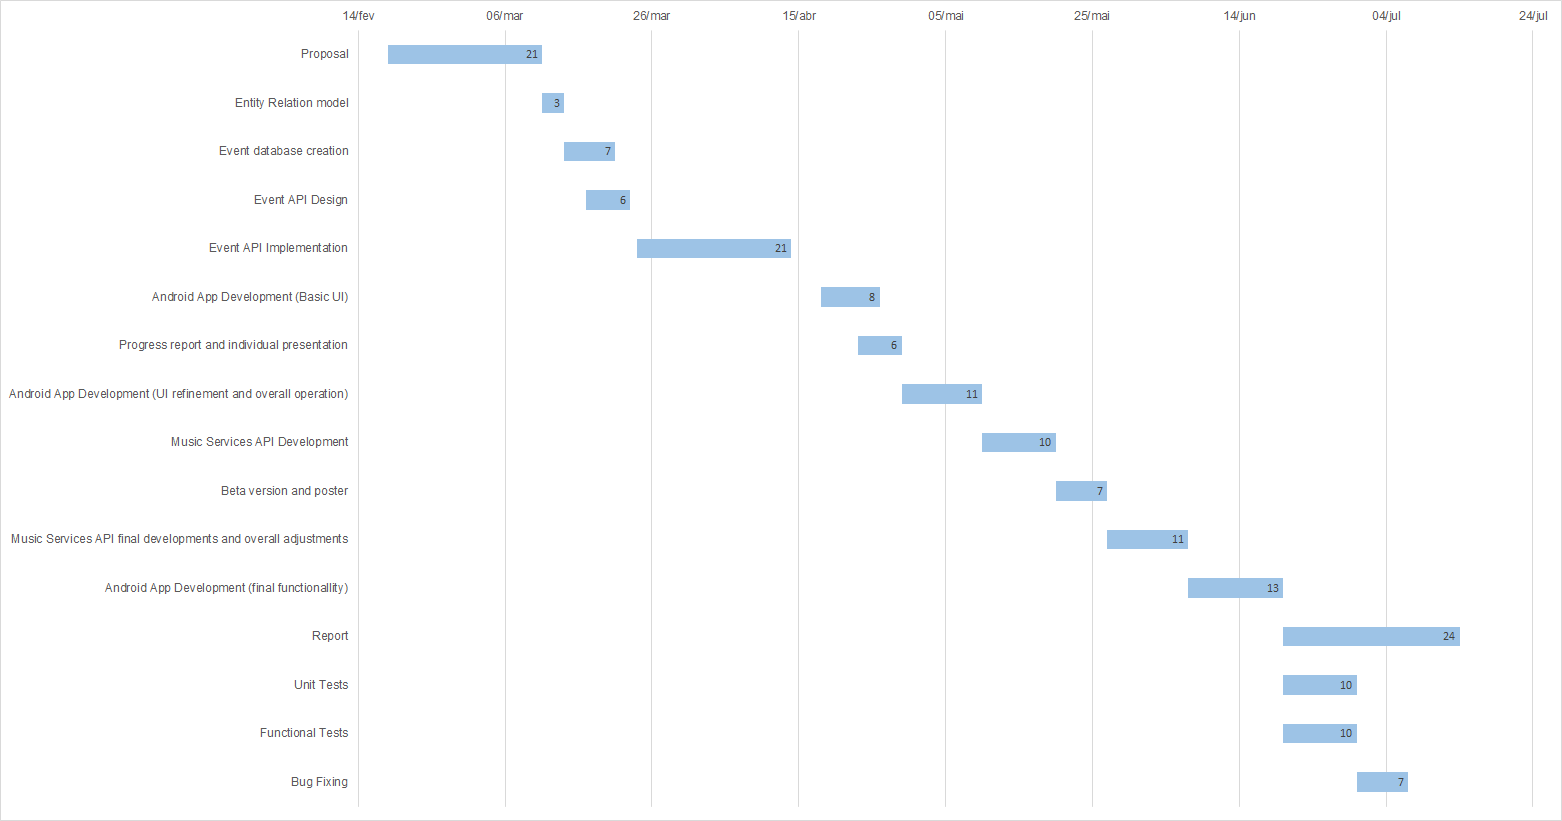
\includegraphics[width=0.75\textwidth]{./Chapter5/Figures/planning.png}
	\caption{Gantt diagram depicting the project plan.}
	\label{fig:GanttDiagram}
\end{figure}

%For now the roadmap the group planned has been successfully followed. Some key parts of the project are still missing but the development tasks are defined to still follow the roadmap and the project is structured so features are added to it.%

%There is now a clearer vision of what the project will be, as the group is now completly sure of the technology that it's using, such as Xamarin Forms instead of Xamarin Native for the Client Application Development, OAuth2 for user authentication, or PostgreSQL as the database engine.%

%However there was a decision to change some of the project structure as development goes, as the group has now a better, more precise view of what the project will end up like.%



